\section{Preliminaries (2 pages)}

%\subsection*{Components}

We model open distributed systems as compositions of primitive components.
Superficially, we recognize two kinds of components: rational components and irrational components.
Intuitively, only the behavior of the former can be finitely represented; that of the latter not.
Components cannot recognize themselves or others as being rational or irrational.
We use irrational components as primitives to model unpredictable environments.

\paragraph{Components}

Each component has a fixed number of ports.
A port can be thought of as a gateway, passing data in and out.
Components without ports are sealed and can no longer be composed.
Semantically, we define the behavior of a component as a (non-well-founded) relation among its ports.
Only rational components harbor finite representations of their behavior.
See figure \ref{fig:Components}.
\begin{figure}[t]
\begin{centering}
\subfloat[\label{fig:Components}Components]{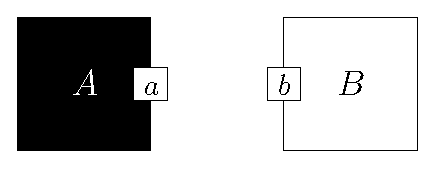
\includegraphics[scale=0.6]{pic/black-white-components}}$\qquad$\subfloat[\label{fig:Channels}Channels]{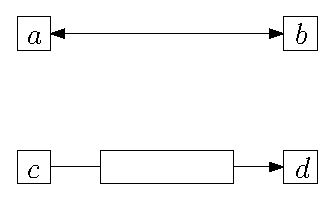
\includegraphics[scale=0.6]{pic/ports-channels}}$\qquad$\subfloat[\label{fig:Node}Node]{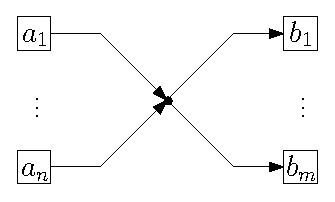
\includegraphics[scale=0.6]{pic/nodes}

}
\par\end{centering}
\caption{
	A black box depicts an irrational component;
	a white box depicts a rational component.
	Channels are pictured by different edge styles.
	Nodes are depicted by black dots,
	merging ports $a_1,...,a_n$ and replicating ports $b_1,...,b_m$.}
\end{figure}

Studying ports is important.
One may stand\textemdash quite literally\textemdash next to a port and observe all data that it passes along.
Sometimes one observes no activity at all, which we denote by $*$.
Other times one observes a datum exchanged through the port, which we leave uninterpreted.
A port is characterized by the set of streams of activity,
where each element is an acceptable stream of observations.

For example, let $a$ be a port. We write $(*,d_{1},*,*,d_{2},\ldots)\in a$, where $d_{1}$ is the first datum observed, $d_{2}$ is the second datum observed, and so on.

\medskip

This work is based on Reo: a language of concurrent protocols and components.
The most important elements of this language are channels, nodes and compositions.
Channels and nodes are primitive components relating data \emph{flows}.
We will later explain two examples of the channels that appear in figure \ref{fig:Channels}.
Nodes are used to link multiple channels together, see figure \ref{fig:Node}.
Finally, composition identifies the shared ports in complex constructions of channels and nodes,
see section \ref{sec:Streams}.

\paragraph{Protocols}

We introduce protocol as a fundamental concept for modeling systems.
Formal protocols are a generalization of formal languages,
in the sense that formal languages define word membership,
whereas formal protocols define stream membership.
We will limit ourselves to $\omega$-regular protocols.

Let $\mathbb{N}$ be the set of natural numbers.
Let $D$ denote a set of data elements.
We leave $D$ uninterpreted, although it is possibly structured in an application-specific way.
We let $\Sigma$ be our alphabet, defined such that $D\subseteq\Sigma$ and $*\in\Sigma$.
We explicitly mention that $*\not\in D$. We often consider constructions
such as pairs $\Sigma\times\Sigma$ which forms a new alphabet with as elements ordered pairs.

A finite sequence, or \emph{word}, is formed by juxtaposing symbols from $\Sigma$.
The set of all words is denoted $\Sigma^{*}$.
A formal language $\mathcal{L}$ is a subset thereof,
i.e. $\mathcal{L}\subseteq\Sigma^{*}$.

An infinite sequence, or \emph{stream}, is formed by an infinite juxtaposing of symbols from $\Sigma$.
The set of all streams is denoted $\Sigma^{\omega}$.
Streams are informally described as infinite tuples
of the shape $(x_{0},x_{1},x_{2},\ldots)$, where each $x_i \in \Sigma$.
A stream is isomorphic to a function $\sigma:\mathbb{N}\to\Sigma$;
a stream $\sigma = (\sigma(0),\sigma(1),\sigma(2),\ldots)$ has
an \emph{initial value} $\sigma(0)$,
and a \emph{stream derivative} $\sigma' = (\sigma(1),\sigma(2),\ldots)$,
and can be specified by differential stream equations \cite{?}.

\medskip

By $\Sigma^{\omega}$ we mean the set of streams of observations.
We will build more complex constructions out of data streams;
$(\sigma_1,\sigma_2)\in \Sigma^\omega\times \Sigma^\omega$ is a pair of streams,
and $(\Sigma\times \Sigma)^\omega$ is the set of streams of pairs.
We can generalize this construction;
$(\sigma_1,\ldots,\sigma_n)\in(\Sigma^\omega)^n$ is an $n$-tuple of data streams,
and $(\Sigma^n)^\omega$ is the set of streams of $n$-tuples of data elements.

We characterize the behavior of a rational component by a relation on data streams.
Consider that $n$-ary relations are \emph{sets} of $n$-tuples of data streams,
i.e. $R\subseteq (D^\omega)^n$ and we have that $(\sigma_{1},\ldots,\sigma_{n})\in R$.
Let $\pi_i(\sigma_{1},\ldots,\sigma_{i},\ldots,\sigma_{n})=\sigma_{i}$ denote tuple projection.
We define relation projection $\Pi_i R$ such that $\sigma_i\in\Pi_i R$ if and only if $(\sigma_{1},\ldots,\sigma_i,\ldots,\sigma_{n})\in R$ where $1\leq i\leq n$.

As a convention, we will consider a rational component and the relation specifying its behavior
to be the same, often denoted by $R$.

\paragraph{Ports}
Intuitively, one can compare our treatment to relational algebra.
In relational algebra, each element of a tuple is named by an attribute name.

Let $P$ denote a countably infinite set of port variables.
Let $P_R$ be the port variables of component $R$.
We use $P_R$ as attribute names of the relation $R$: for $P_R=\{a,b,\ldots\}$, we often write $R(a,b,\ldots)$. We characterize a port $v\in P_R$ by the set of data streams $\Pi_v R$, by abusing notation of $\Pi$.

Equivalent up to isomorphism, and more convenient for our purposes,
let the $n$-ary relation $R$ be sets of streams of $n$-ary tuples of data,
that is, $R\subseteq (D^n)^\omega$.

\begin{table}[b]
	\begin{center}
		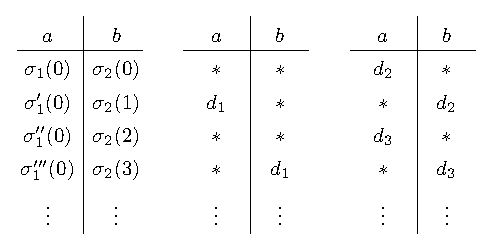
\includegraphics[scale=0.8]{pic/stream-table}
	\end{center}
	\caption{
		\label{fig:Stream-Table}Left-most table shows stream notation. Other tables are example observations that are in $A(a,b)$.  Each column is a stream associated to a port variable: we have that $\Pi_a A(a,b)=\sigma_1$ and $\Pi_b A(a,b)=\sigma_2$. Intuitively, each table describes a pair of streams, and a stream of pairs.}
\end{table}

We illustrate these concepts more concretely in Table \ref{fig:Stream-Table}.
Note that such a table only illustrates a \emph{single} stream of $n$-tuples as its rows.
In summary, a component is characterized by a \emph{set} of acceptable tables,
and its port are characterized by the (set of) columns of such tables.

\vspace{-5pt}

\paragraph{Channels} We consider two channels: synchronous and asynchronous,
as depicted in figure \ref{fig:Channels} respectively at the top and the bottom.
We specify the behavior of a synchronous channel between ports $a$ and $b$, denoted $S(a,b)\subseteq(\Sigma\times\Sigma)^{\omega}$, as the largest relation such that:
$$\sigma\in S(a,b)\Leftrightarrow\left[\exists d\in \Sigma.\,\sigma(0)=(d,d)\right]\land\sigma'\in S(a,b)$$
that is, the two ports have equal data streams.

We now specify the behavior of an asynchronous channel, of which two examples are shown
in Table \ref{fig:Stream-Table}. An asynchronous channel between ports $a$ and $b$ is denoted $A(a,b)\subseteq(\Sigma\times\Sigma)^{\omega}$,
as the largest relation:
\begin{align*}
	\sigma\in A(a,b)\Leftrightarrow\exists d\in \Sigma.\, & \sigma(0)=(d,*)\,\land\\
	& \exists i.\,\sigma(i)=(*,d)\land\left[\forall j<i.\,\sigma(j)=(*,*)\right]\,\land\\
	& \phantom{\exists i.\,}\sigma^{(i+1)}\in A(a,b)
\end{align*}
for non-zero $j$, and the repeated stream derivative: $\sigma^{(n+1)}=\left(\sigma^{(n)}\right)'$; $\sigma^{(0)}=\sigma$.

Intuitively, an asynchronous channel is either inactive or passes a datum in a delayed fashion.
Let $i=0$ and see that $\sigma(0)=(*,*)$.
If port $a$ offers a datum then port $b$  takes the same datum at some time later,
while both ports remain inactive in the mean time. Note that when $a$ and $b$ are also
connected by a synchronous channel, the behavior collapses into the singleton set accepting only $(*,*,\ldots)$: this is explained in section \ref{sec:Streams}.

In essence there is no difference in the sensing of a port as \emph{input} or \emph{output}.
We only provide such designation to aid the informal description for an intuitive operational understanding. In practice, fixing port sense allows for optimization.

\paragraph{Nodes}

Finally, we specify the node as depicted in \ref{fig:Node}.
Nodes have $n+m$ number of ports with $n,m\geq1$.
Its ports are denoted $a_1,\ldots,a_n$ and $b_1,\ldots,b_m$.
Recall that $\pi_i$ is tuple projection.
The behavior of nodes are characterized by the $(n+m)$-ary relation $N$,
defined as the largest relation such that:
\begin{align*}
	\sigma\in N\Leftrightarrow\,\, & \exists d\in \Sigma.\,
	\bigl[\exists i\leq n.\,\pi_i\sigma(0) = d\land\left[\forall i'\leq n.\,i'\neq i\rightarrow\pi_{i'}\sigma(0) = *\right]\,\land\\
	& \phantom{\forall d\in D.\, \bigl[}\forall j\leq m.\,\pi_{n+j}\sigma(0)=d\bigr]\,\land\\
	& \sigma'\in N
\end{align*}
where $i,i',j$ are non-zero.
Intuitively, nodes are synchronous channels that merge and replicate data.
Merge specifies that at most one of the $n$ channels can offer a datum,
and all others $n$ channels are inactive.
Replication specifies that all of the $m$ channels takes the datum offered.
Also, all ports of a node can be inactive.
